\documentclass[a4paper,12pt]{article}

\usepackage{../usfdvl}


\title{Worksheet 7}
\SetDocumentFooter{}{}


\begin{document}

\maketitle

\worksheetGroundRules


\vspace{5pt}
\section{Assignment}

\begin{itemize}



\item For the following point set, find the Voronoi diagram using the insertion method. Show the algorithm using the following pages. Be sure to show all of the steps and the order of steps for the algorithm (i.e., all of the intersections).

\begin{center}
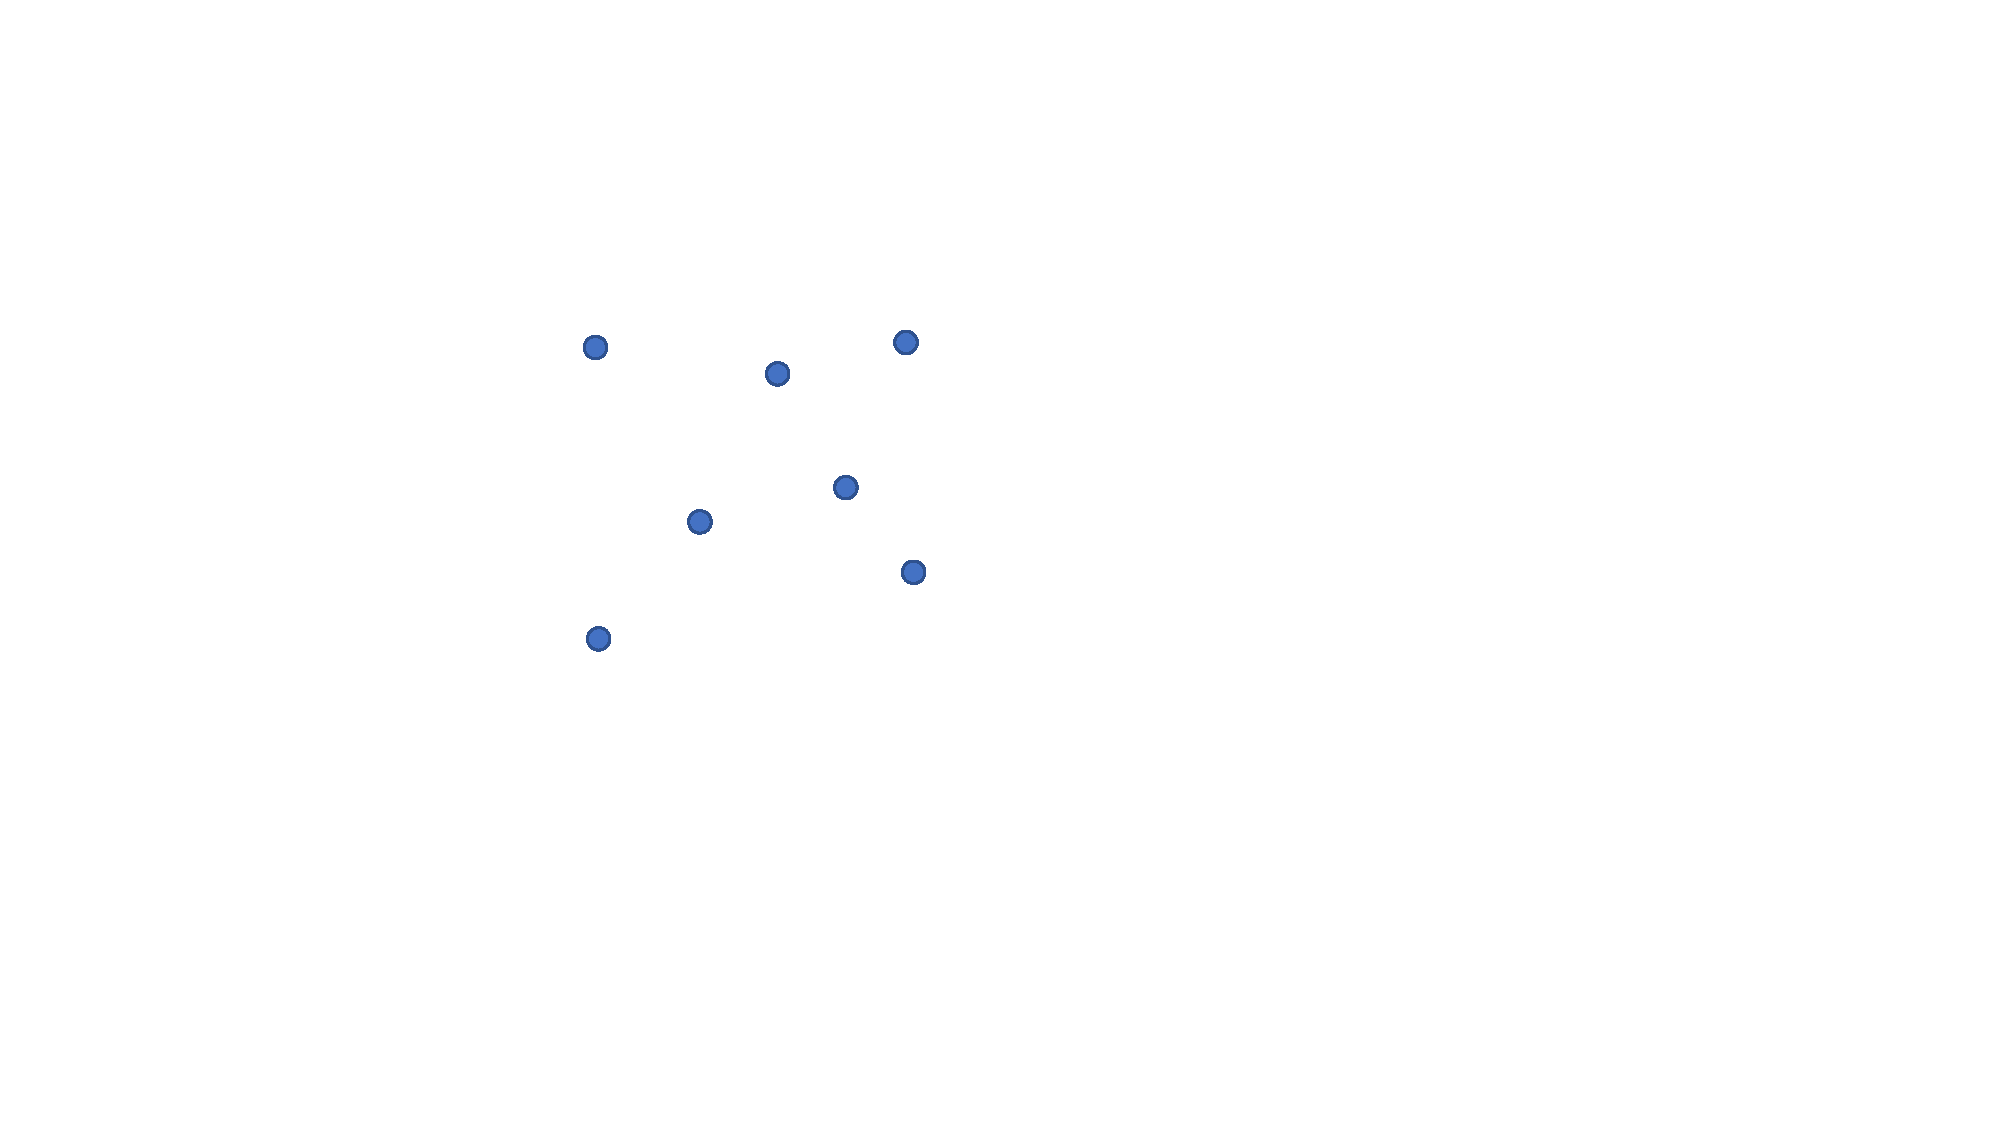
\includegraphics[width=6cm]{../images/voronoi7.pdf}
\end{center}


\item Use each steps to determine the best/average/worst case big-O performance for a single iteration. 
\item Combine that information to determine the best/average/worst case big-O for the entire computation.

\item Using the final Voronoi diagram to determine the Delaunay Triangulation. 

\item Determine the best/average/worst case big-O for the Delaunay Triangulation computation.


\end{itemize}


\worksheetSubmission



\newpage

\begin{tabular}{|c|c|}
\hline
\hspace{10pt}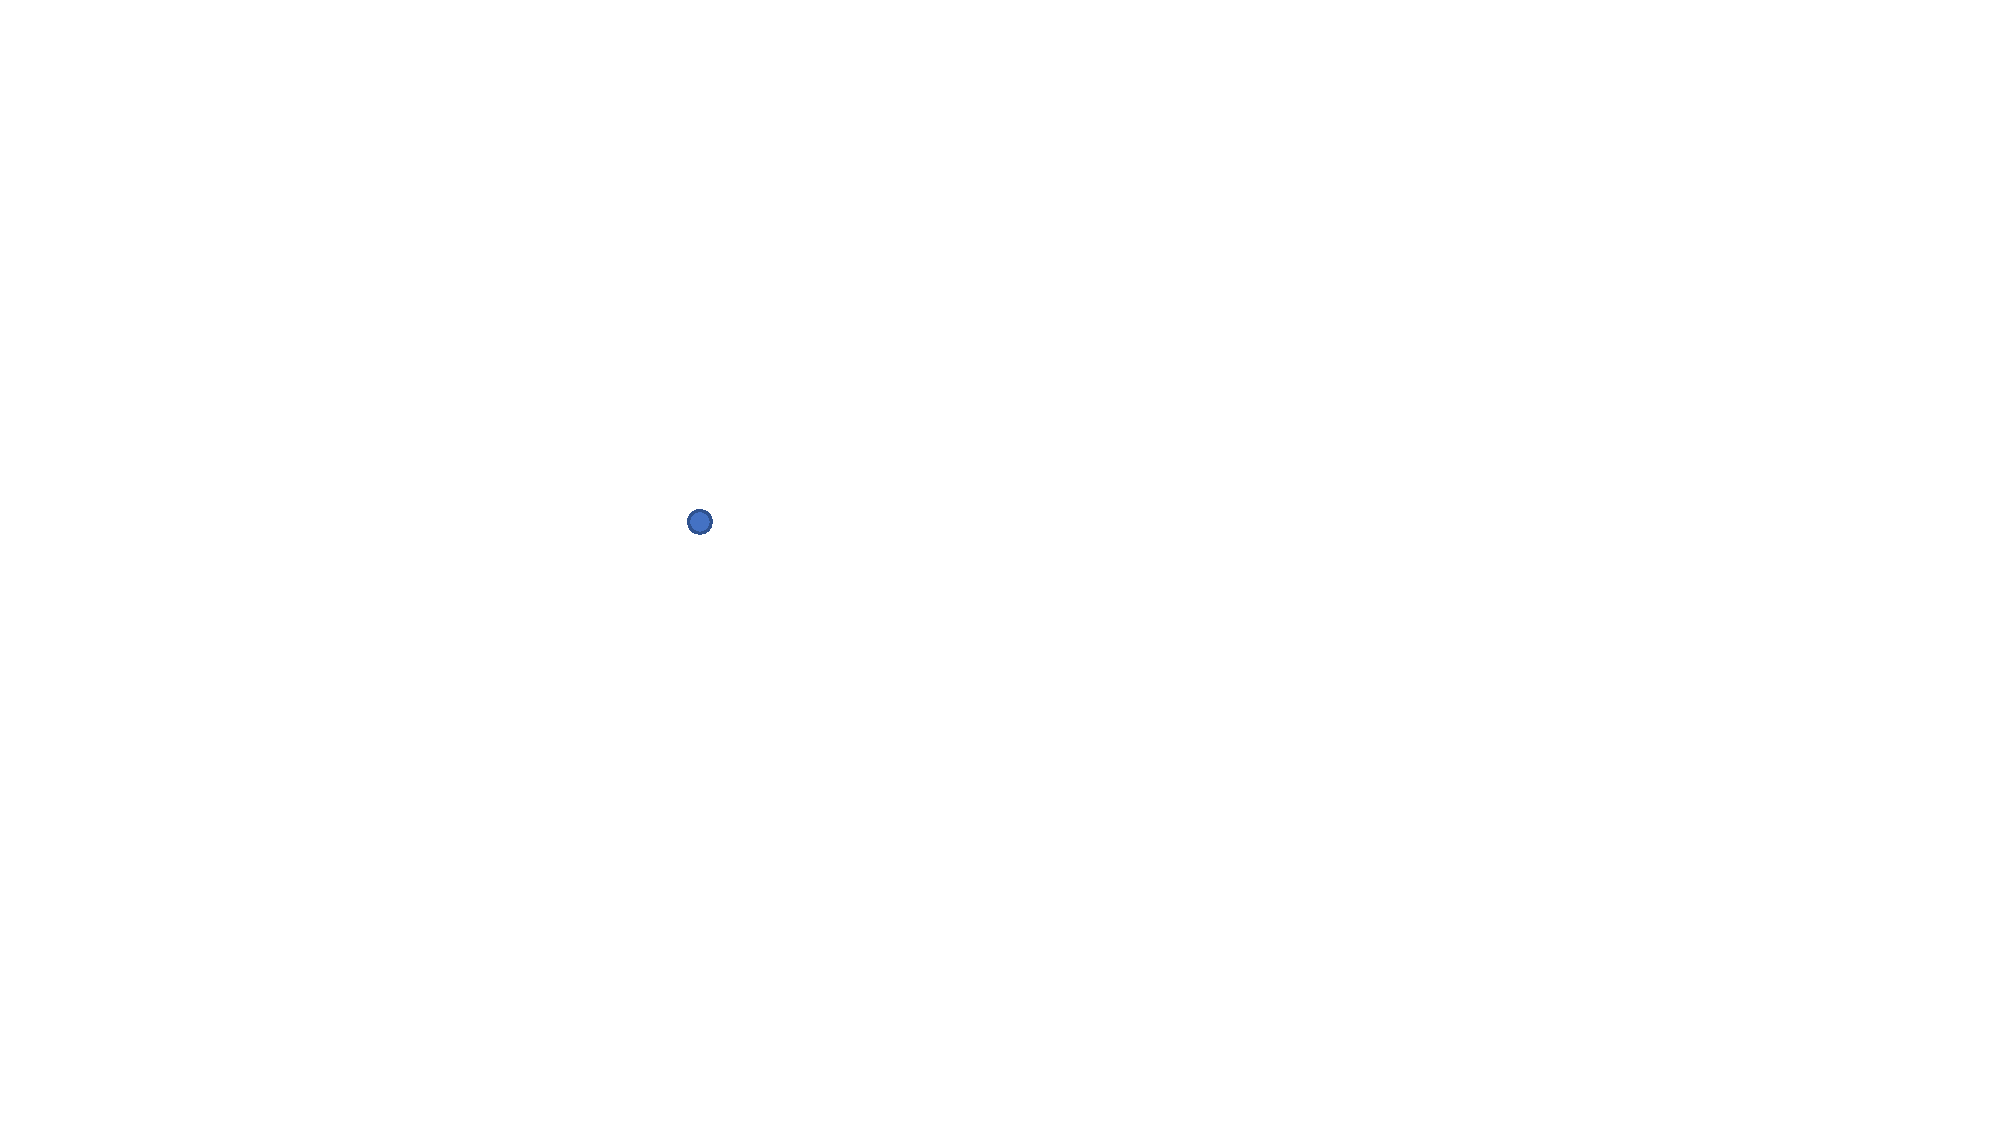
\includegraphics[width=0.425\linewidth]{../images/voronoi1.pdf}\hspace{10pt} & \hspace{10pt}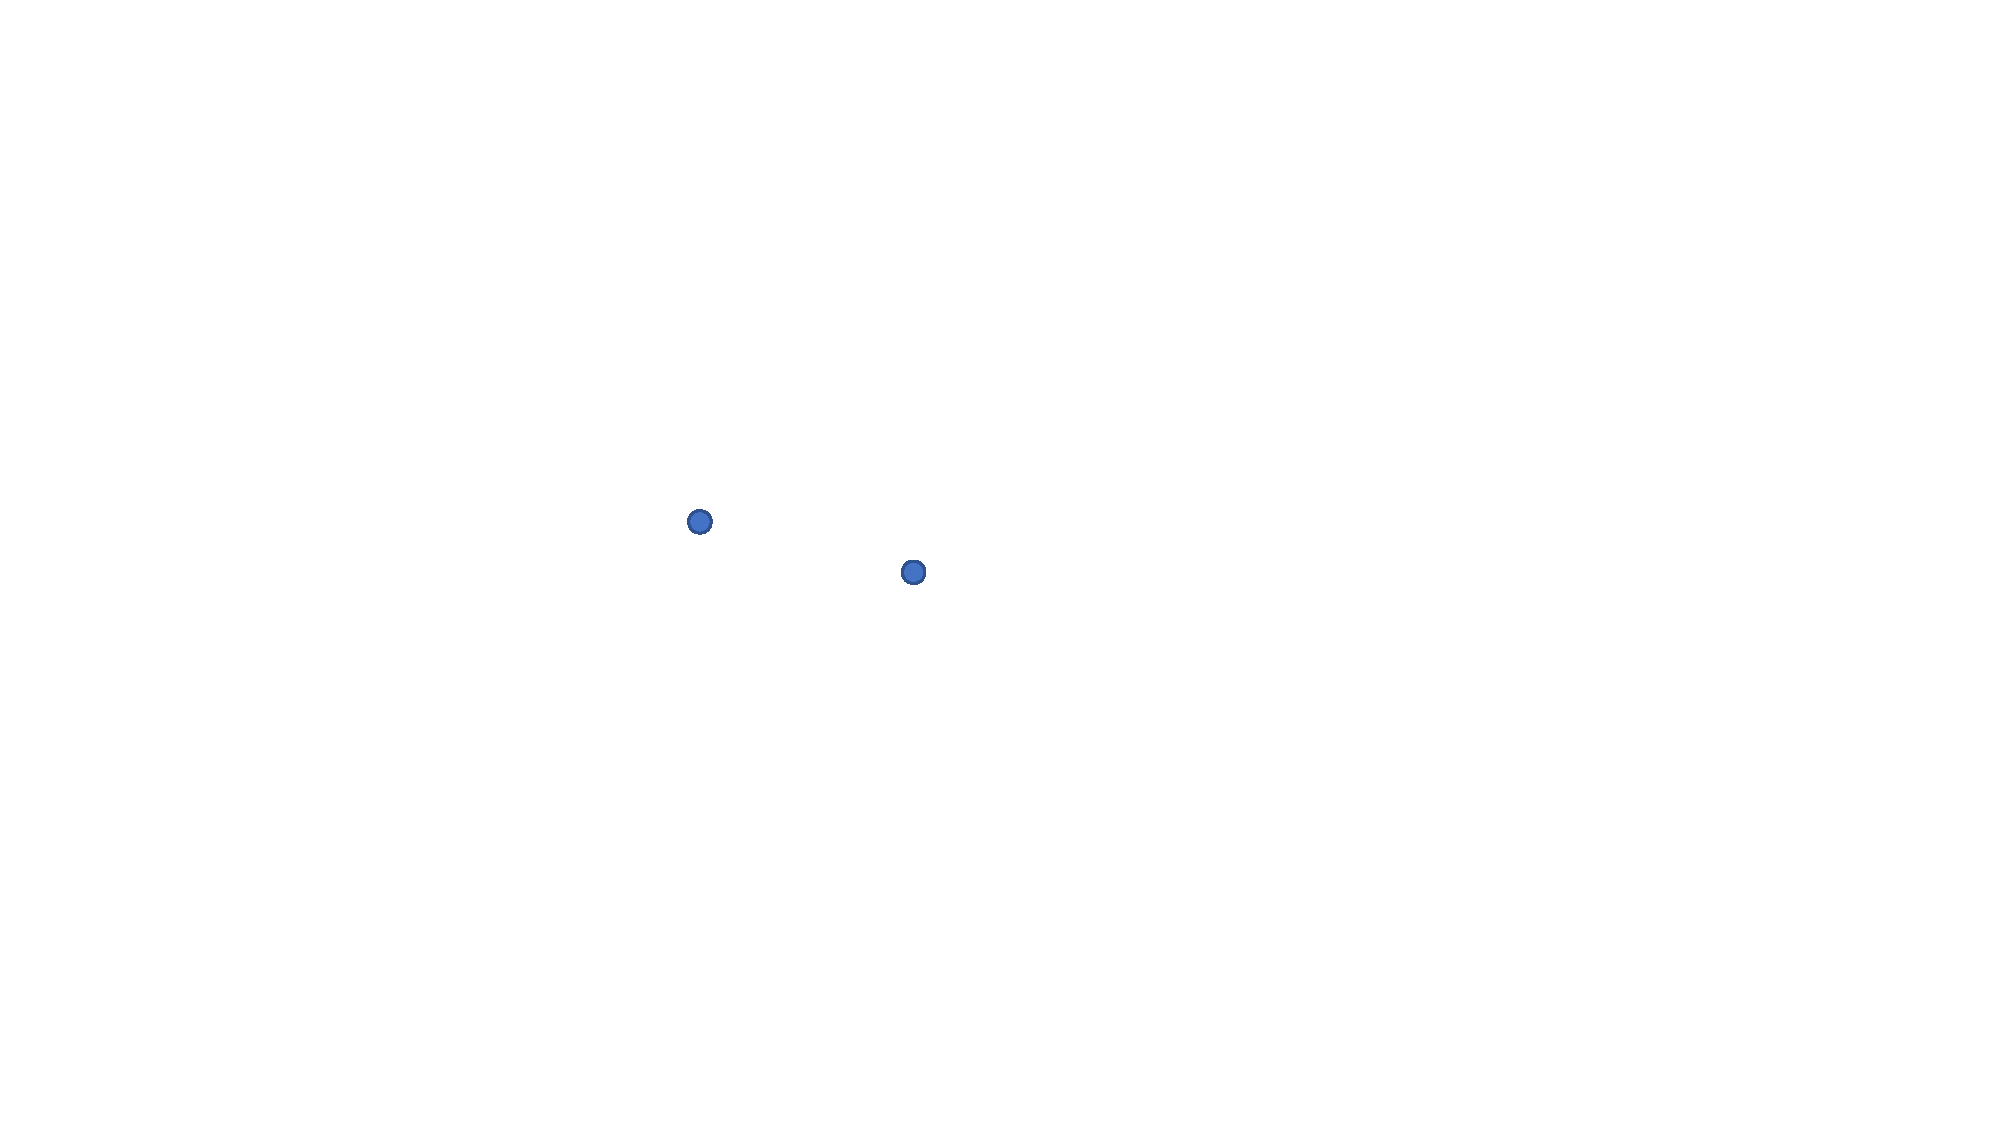
\includegraphics[width=0.425\linewidth]{../images/voronoi2.pdf}\hspace{10pt} \\
Voronoi Diagram & Voronoi Diagram \\
\hline
\hspace{10pt}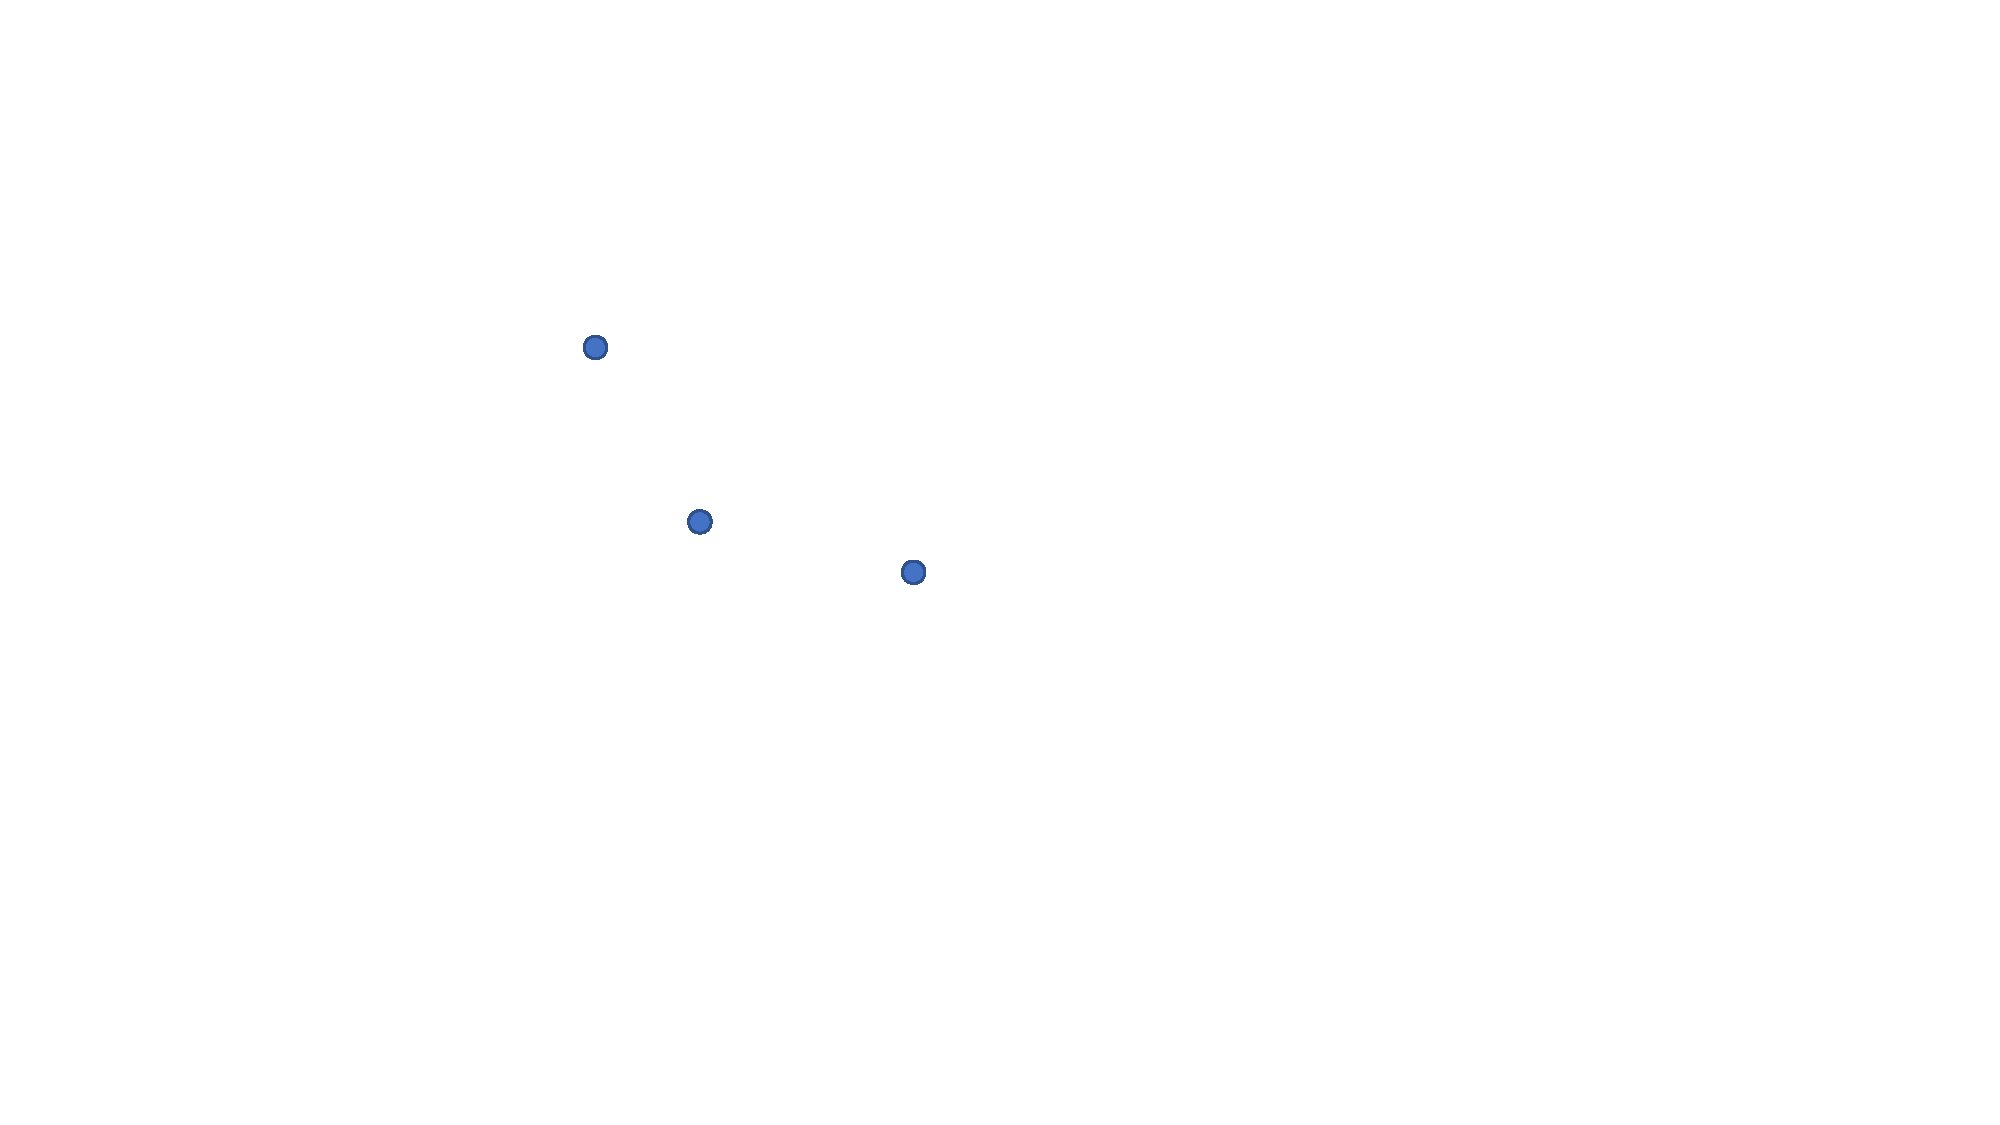
\includegraphics[width=0.425\linewidth]{../images/voronoi3.pdf}\hspace{10pt} & \hspace{10pt}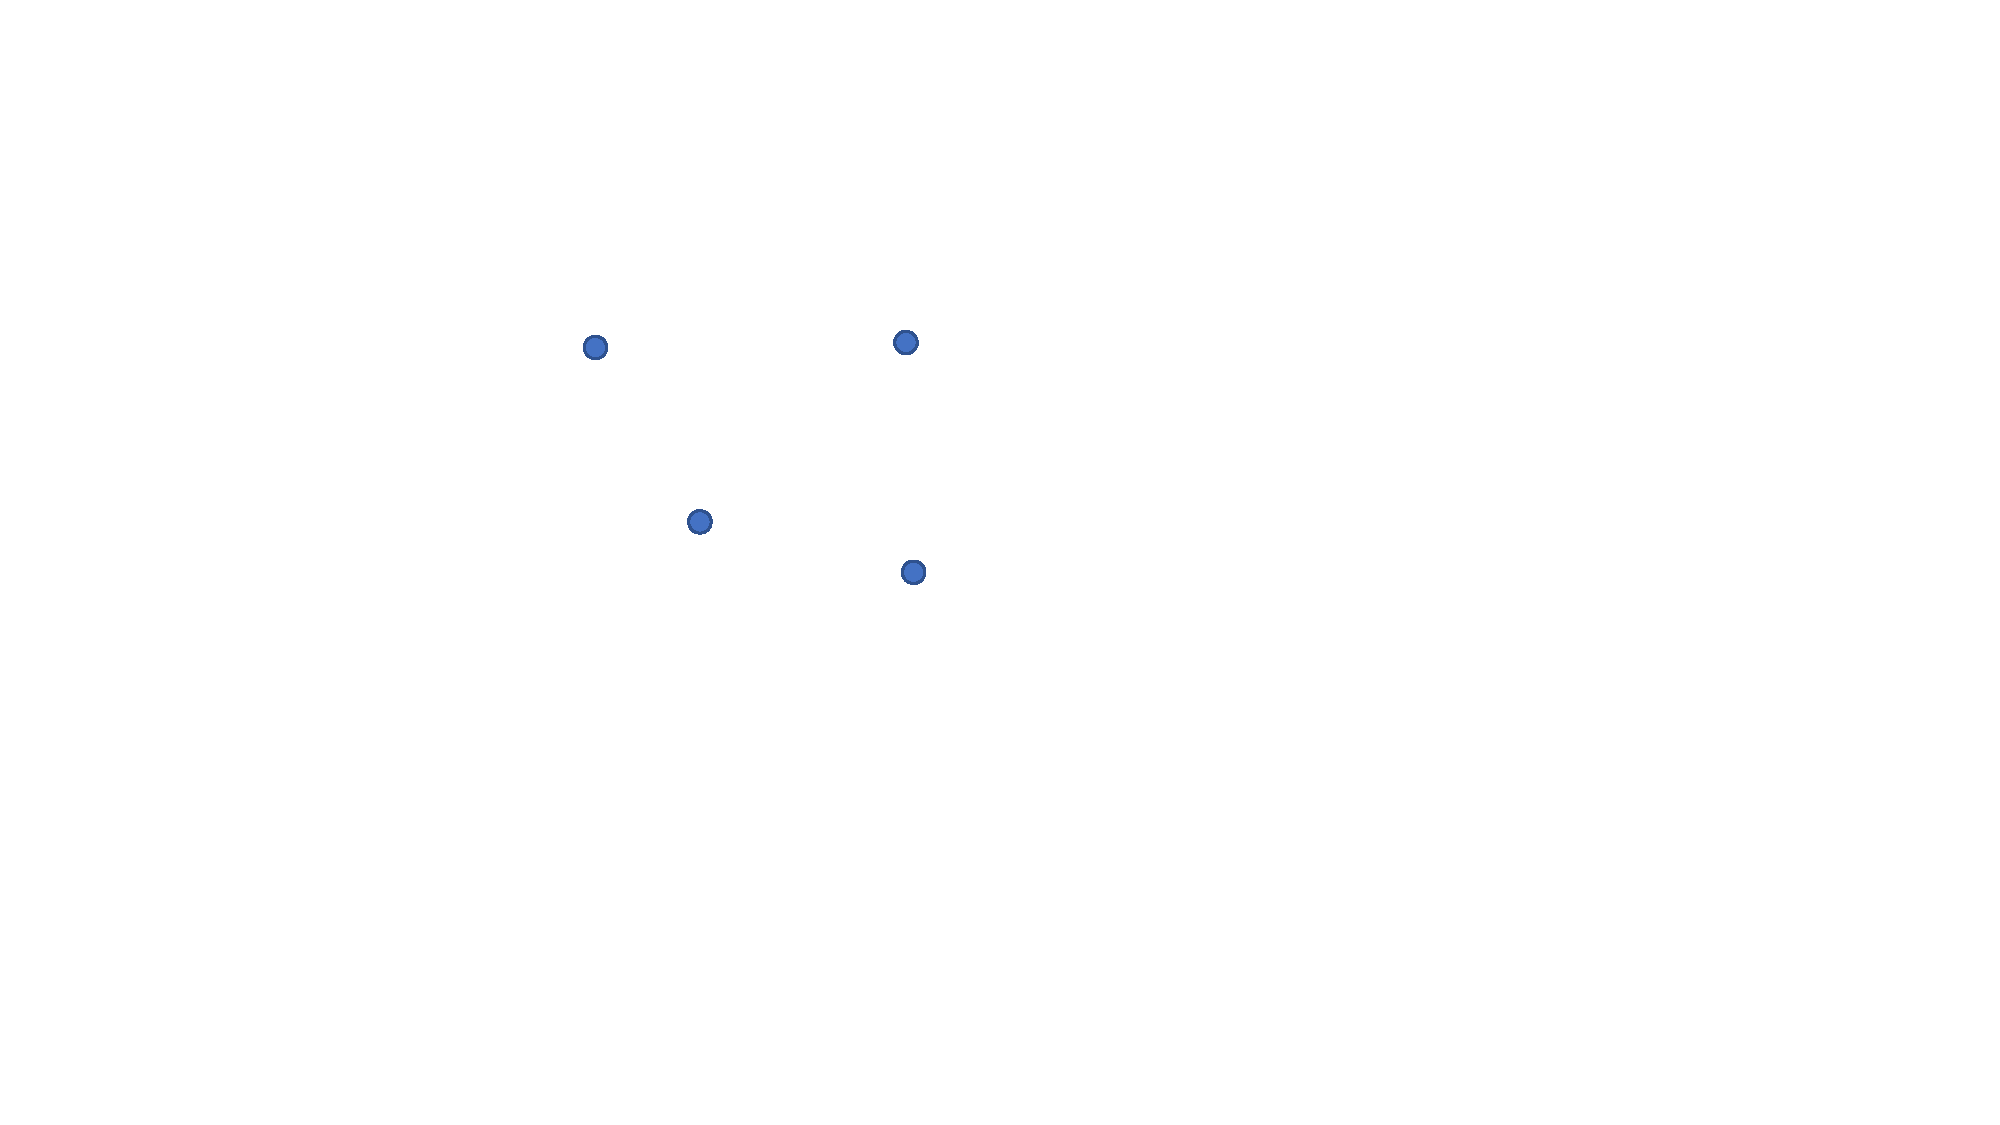
\includegraphics[width=0.425\linewidth]{../images/voronoi4.pdf}\hspace{10pt} \\
Voronoi Diagram & Voronoi Diagram \\
\hline
\end{tabular}

\begin{tabular}{|c|c|}
\hline
\hspace{10pt}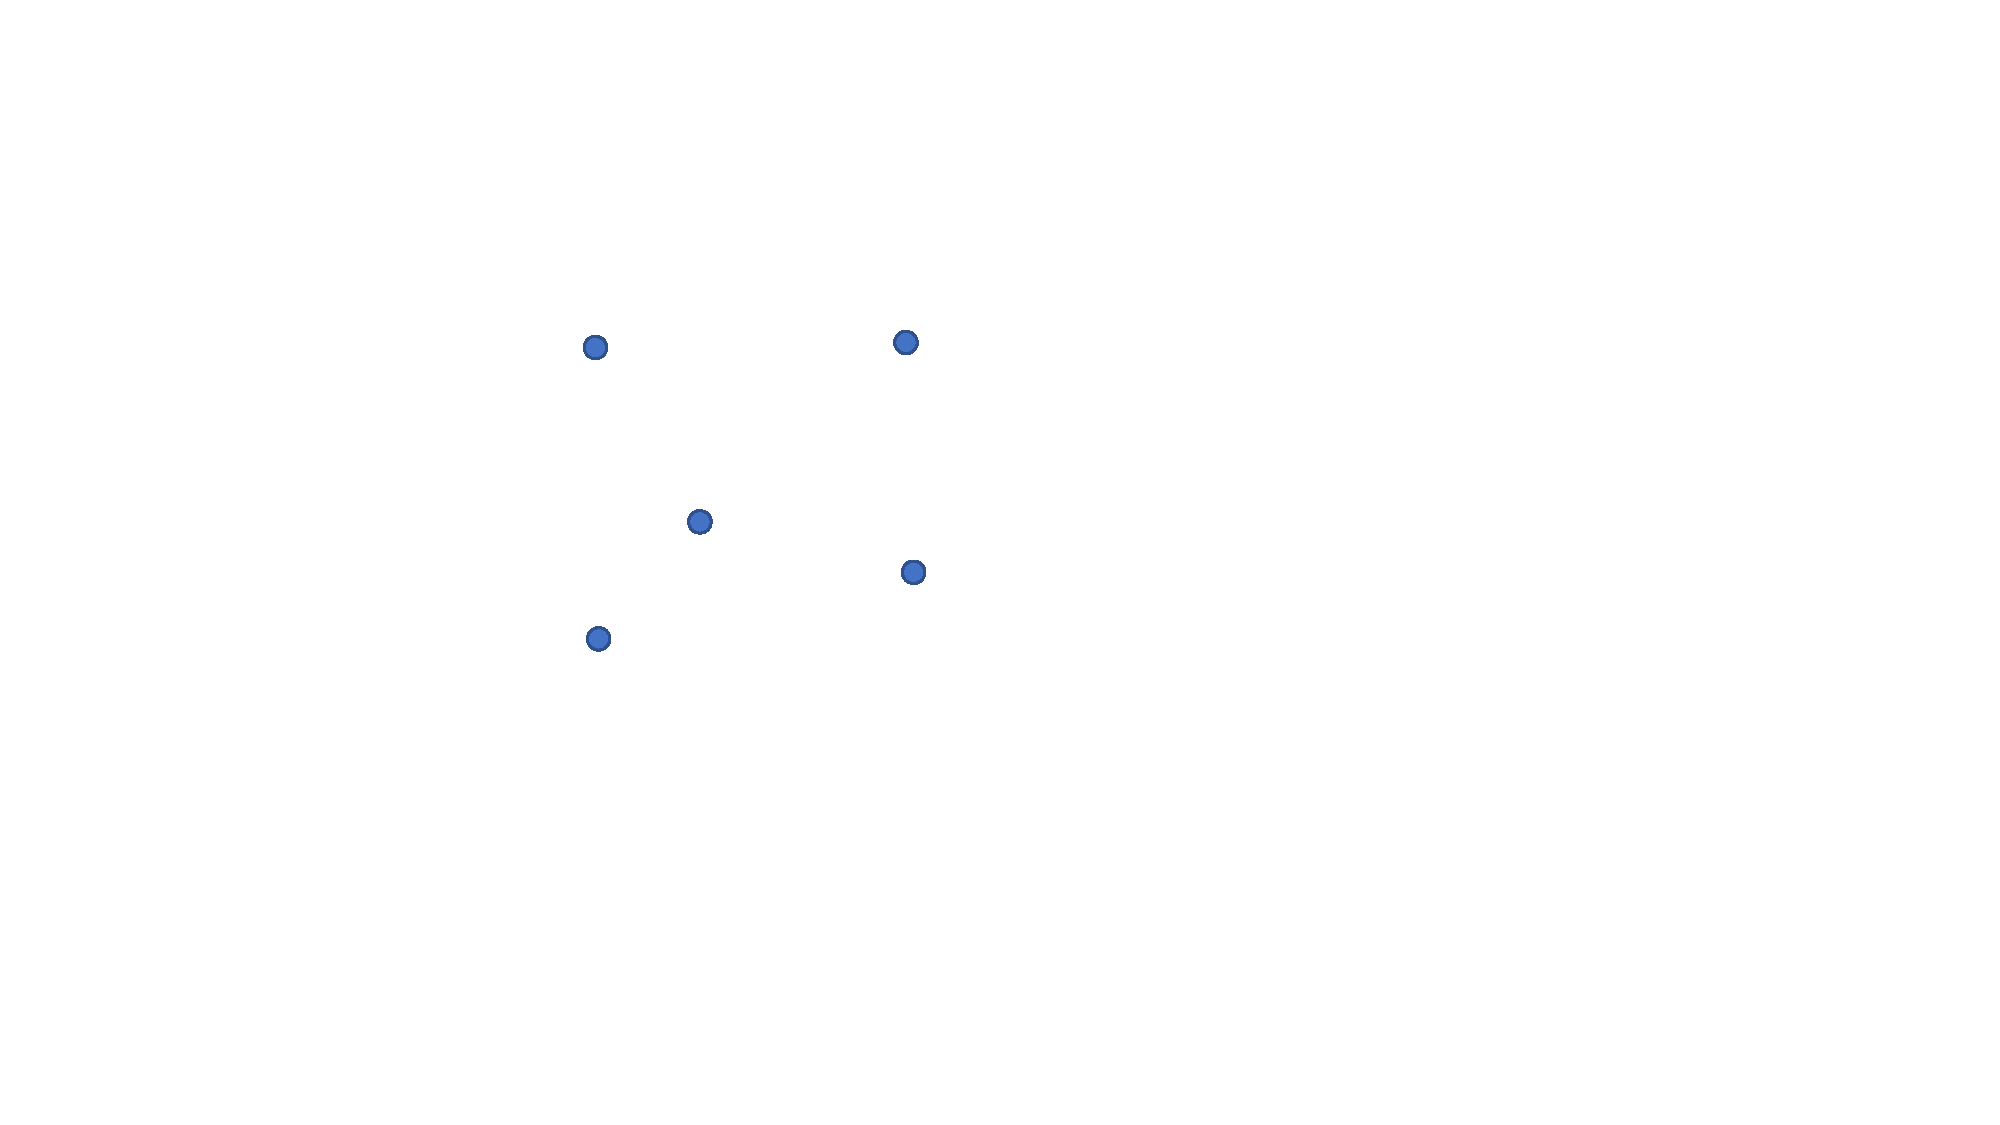
\includegraphics[width=0.425\linewidth]{../images/voronoi5.pdf}\hspace{10pt} & \hspace{10pt}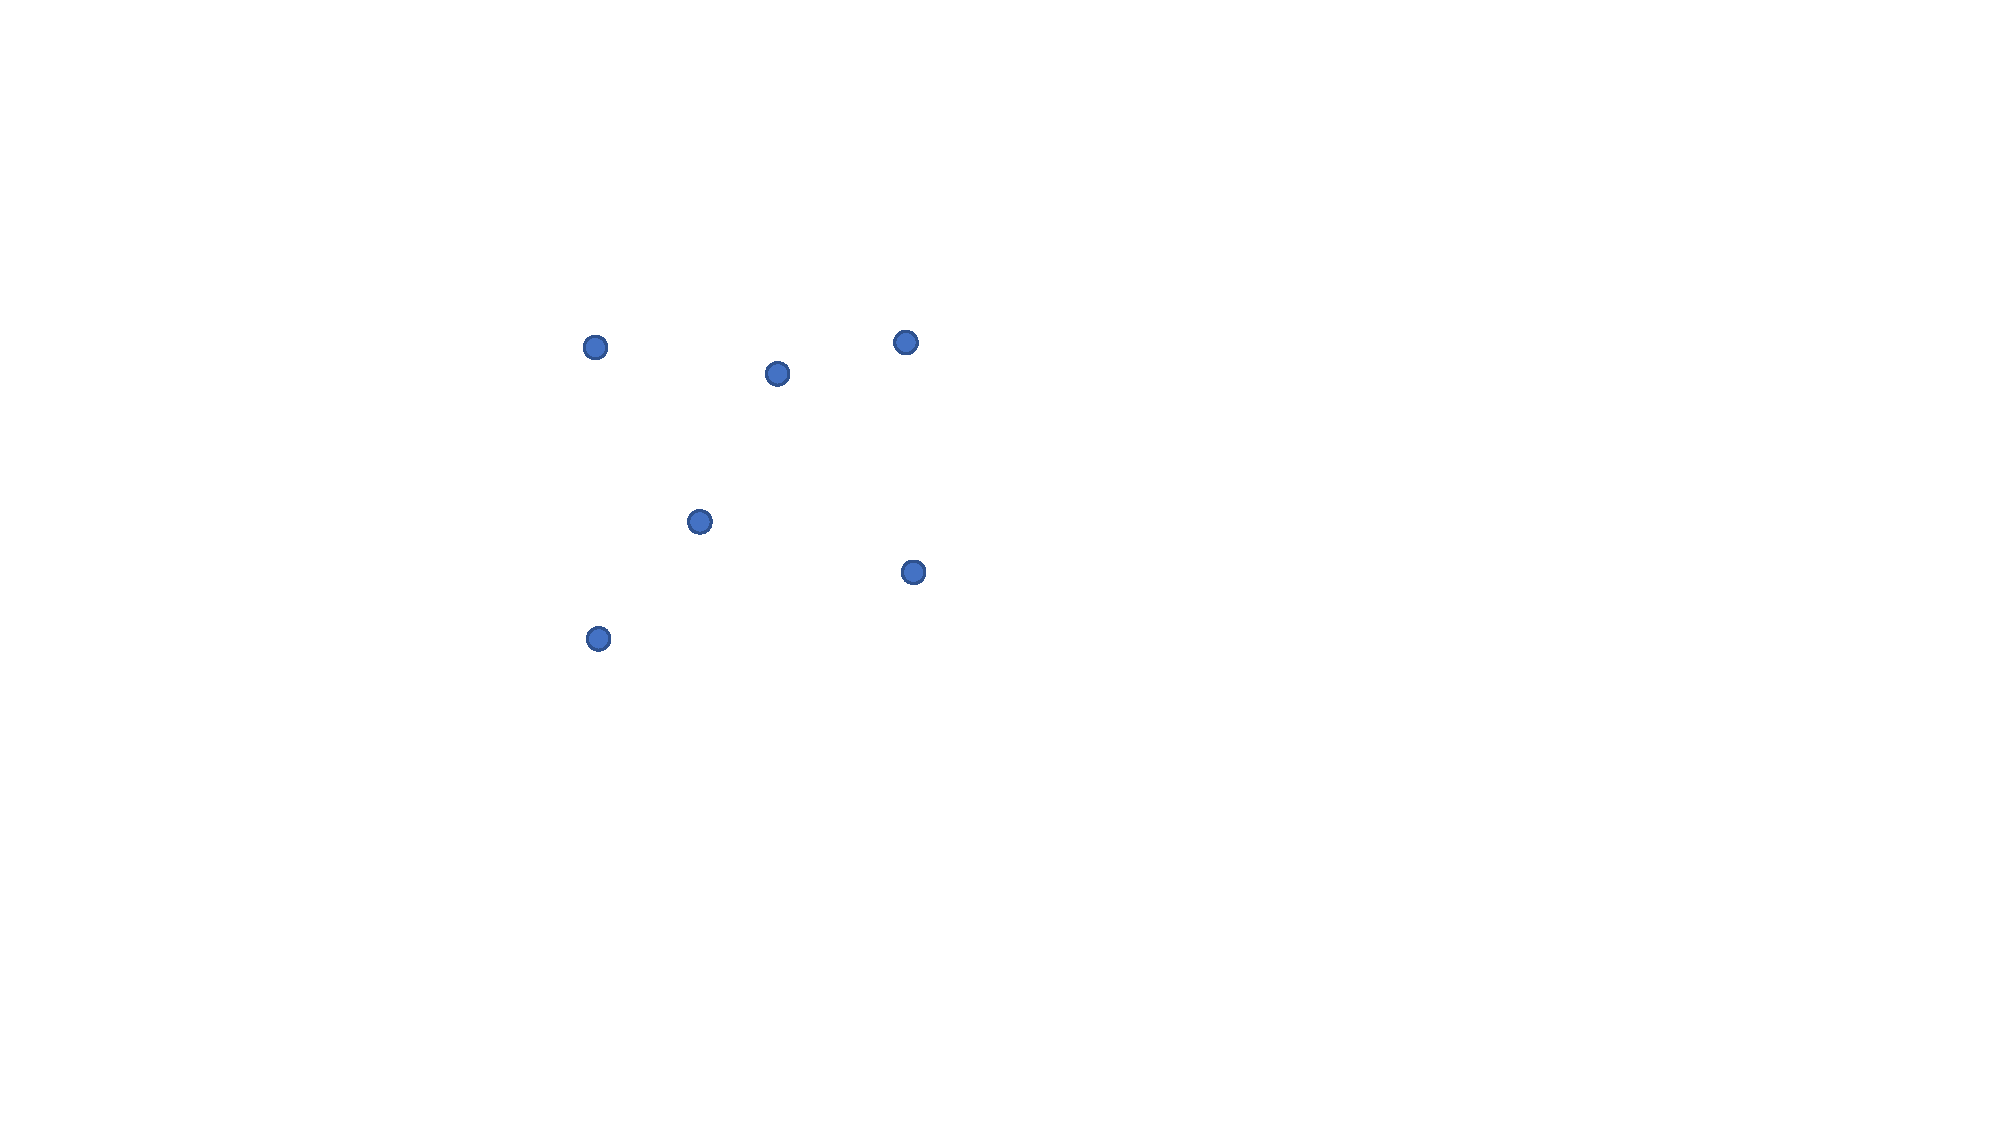
\includegraphics[width=0.425\linewidth]{../images/voronoi6.pdf}\hspace{10pt} \\
Voronoi Diagram & Voronoi Diagram \\
\hline
\hspace{10pt}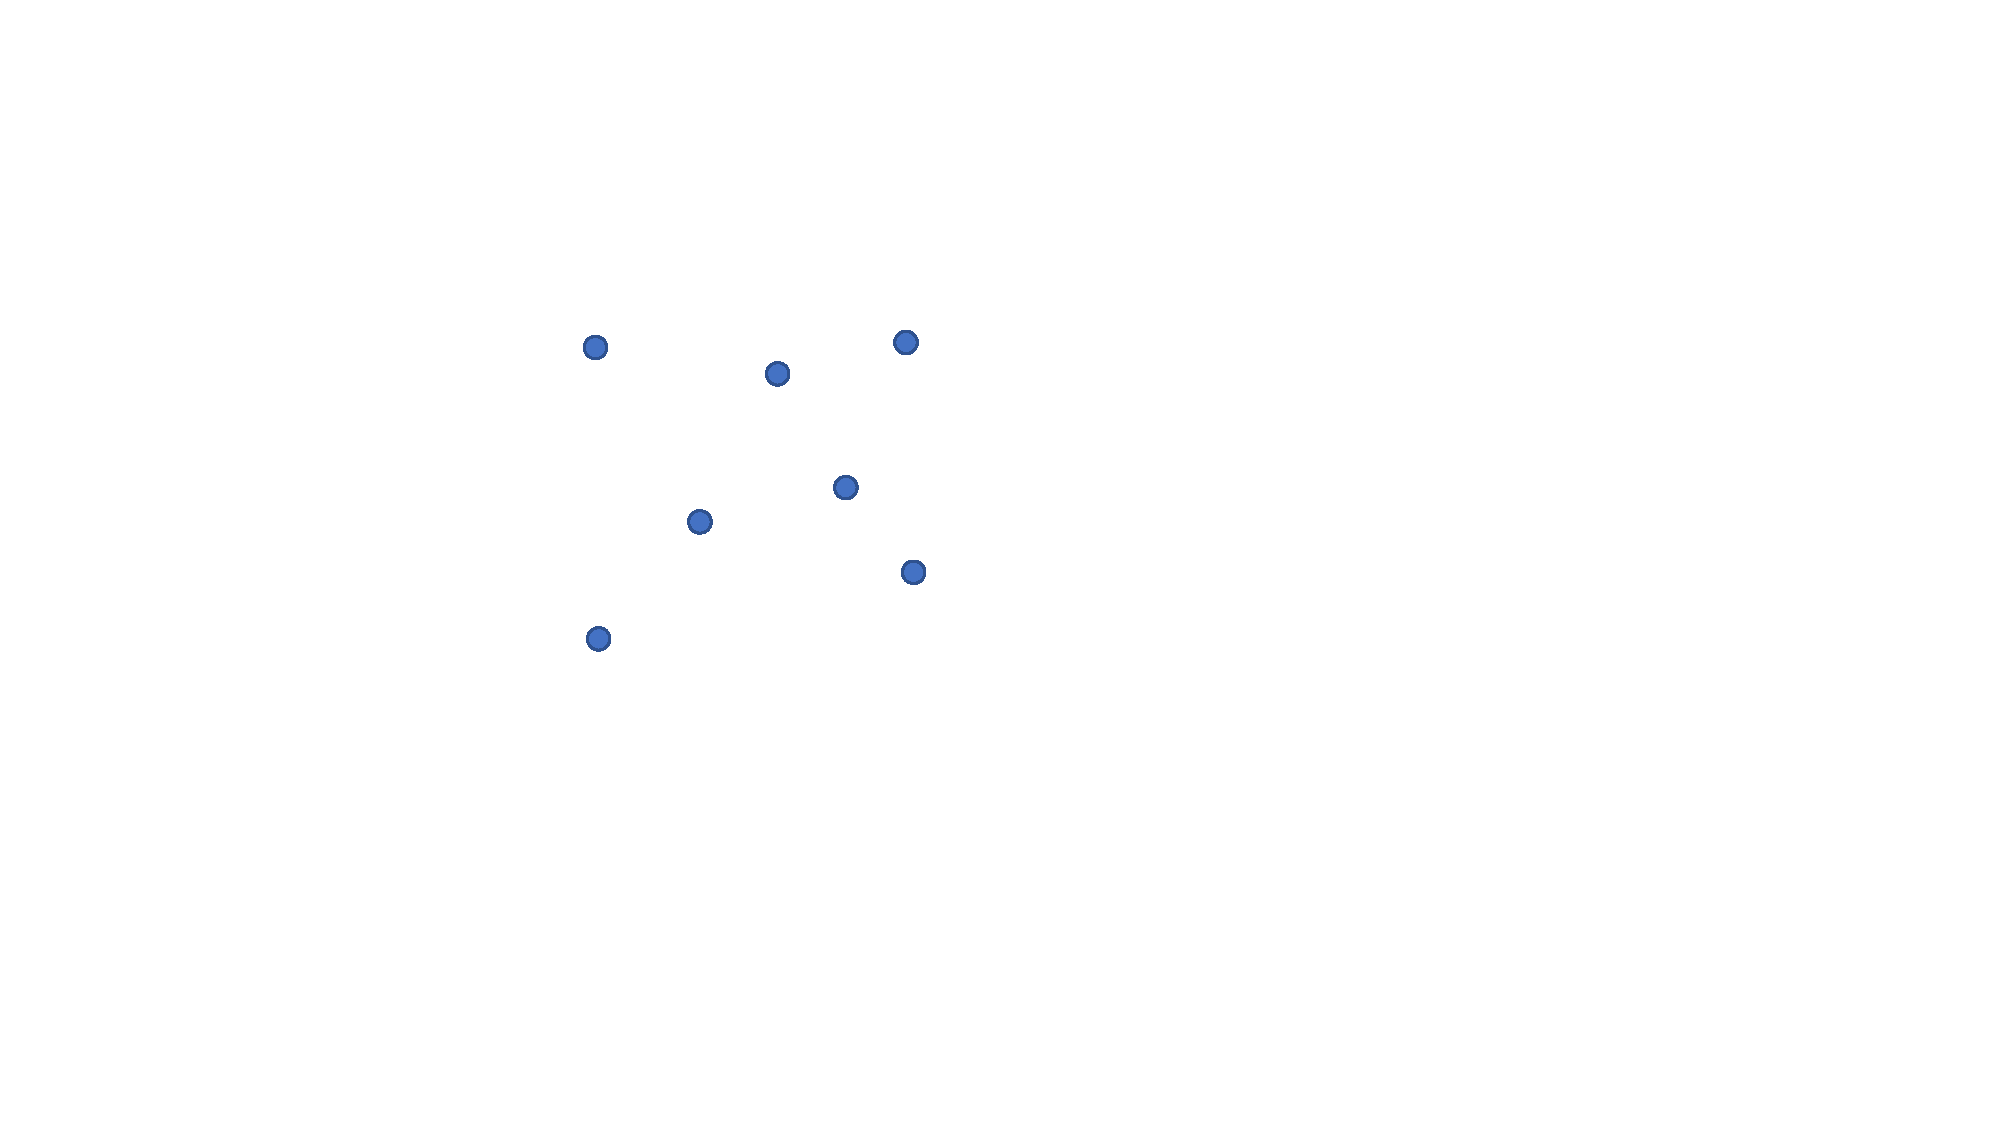
\includegraphics[width=0.425\linewidth]{../images/voronoi7.pdf}\hspace{10pt} & \hspace{10pt}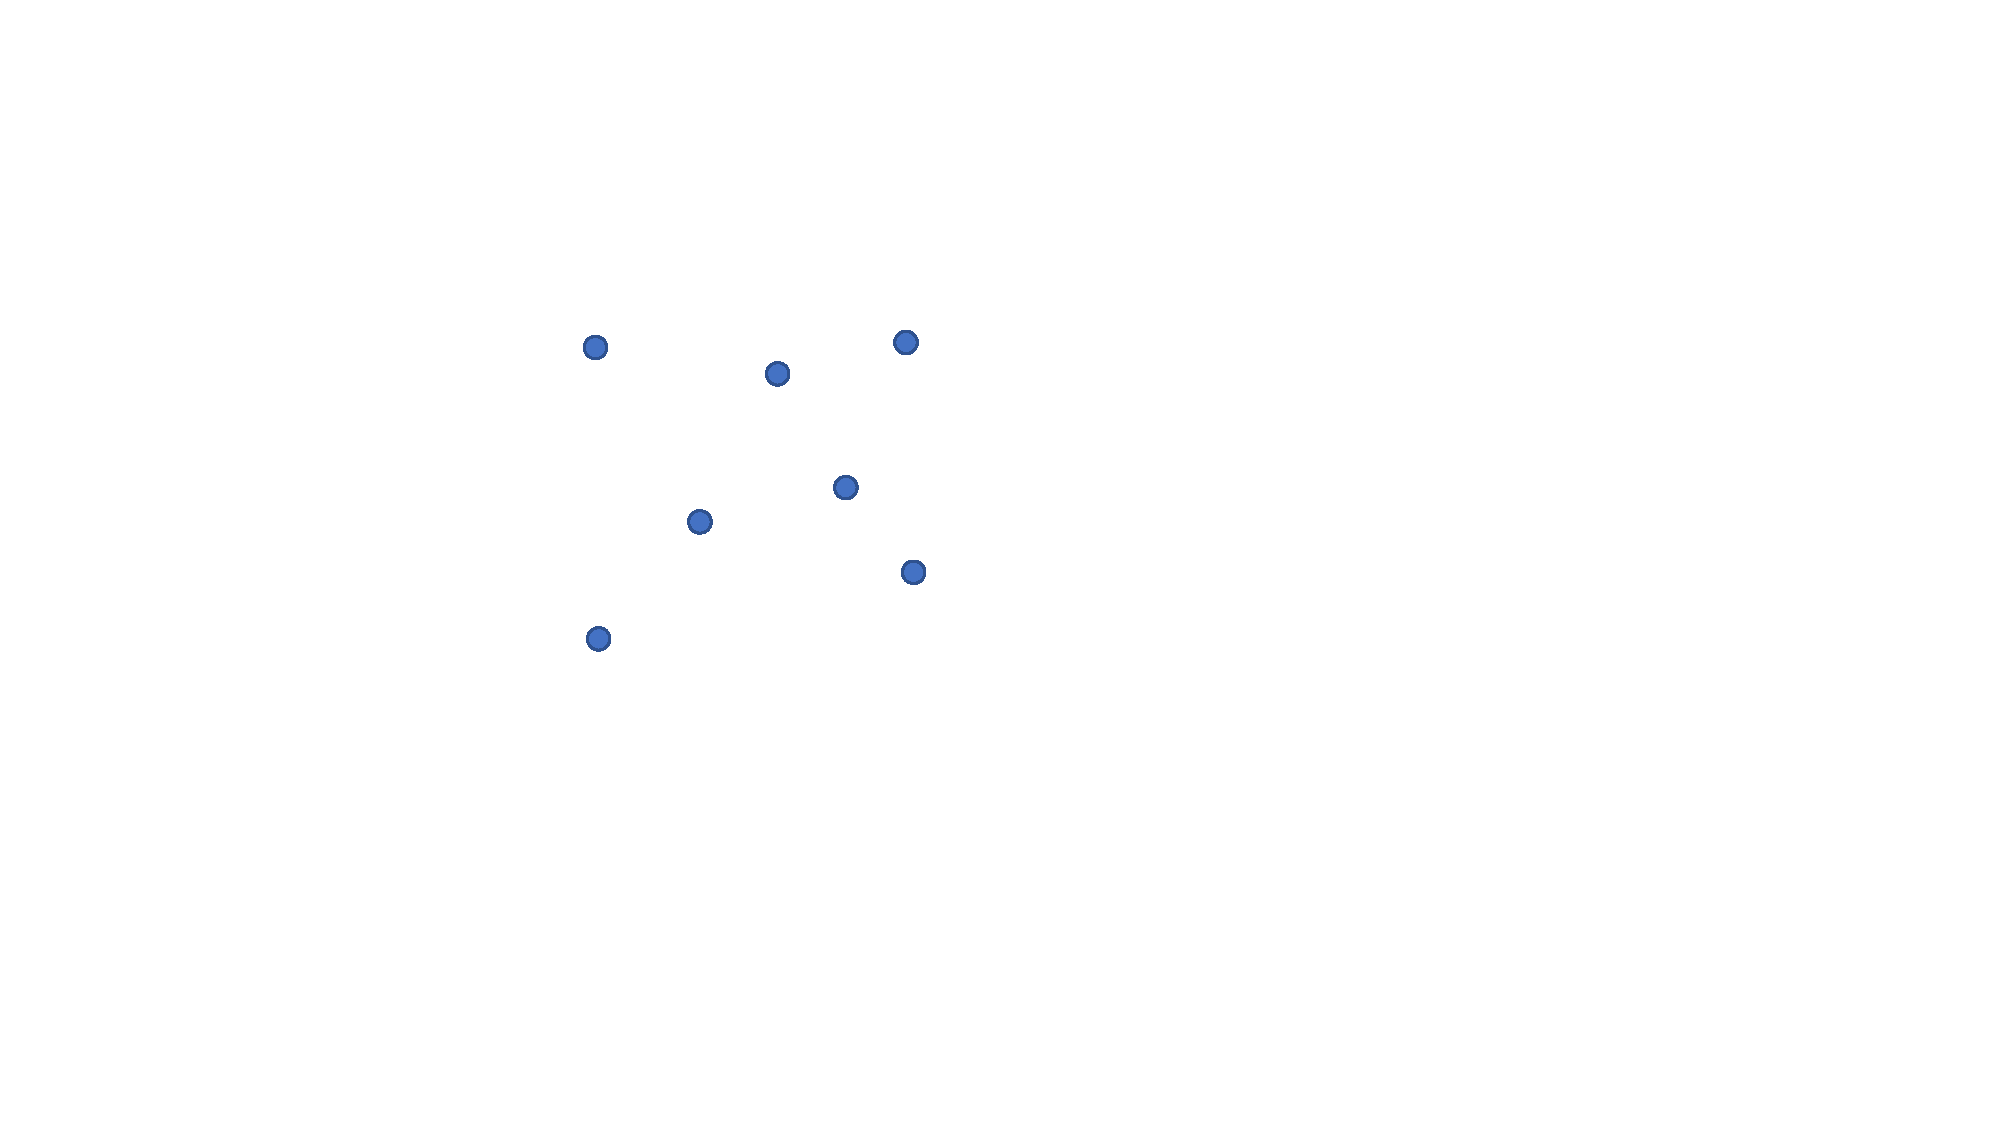
\includegraphics[width=0.425\linewidth]{../images/voronoi7.pdf}\hspace{10pt} \\
Voronoi Diagram & Delaunay Triangulation \\
\hline
\end{tabular}





\end{document}



